%\documentclass[a4paper,doc]{apa6}
\documentclass[a4paper]{article}

\usepackage[english]{babel}
\usepackage[utf8x]{inputenc}
\usepackage{apacite}
\usepackage{authblk}  % for authors

\usepackage{amsmath}
\usepackage{graphicx}
\usepackage[colorinlistoftodos,prependcaption]{todonotes}

\newcommand{\EJ}[1]{\todo[inline, color=green]{  #1 }}
\newcommand{\Q}[1]{\todo[inline, color=yellow]{  #1 }}
\newcommand{\jv}[2]{{\color{red}\st{#1}}{\color{blue}\bf{#2}}}
\newcommand{\DON}[1]{\todo[inline, color=orange]{#1}}

\graphicspath{{../figures/}}
\newcommand{\hypo}{\mathcal{H}}
\newcommand{\model}{\mathcal{M}}

\newcommand{\osflink}{\url{https://osf.io/uq8st/}}

\title{A Cautionary Note on Estimating Effect Sizes with Classical Confidence Intervals}
%\shorttitle{Estimating Effect Size} 
\renewcommand{\thefootnote}{\fnsymbol{footnote}}
\author[1]{Don van den Bergh%
	\thanks{Correspondence concerning this article should be addressed to: Don van den Bergh, University of Amsterdam, Department of Psychological Methods, Nieuwe Achtergracht 129B, 1018VZ Amsterdam, The Netherlands. E-Mail should be sent to: donvdbergh@hotmail.com.
}}
\author[1]{Julia M. Haaf}
\author[1,2]{Alexander Ly}
\author[3]{\authorcr Jeffrey N. Rouder} % putt Jeff on a newline to avoid a newline after his first name
\author[1]{Eric-Jan Wagenmakers}
\affil[1]{University of Amsterdam}
\affil[2]{Centrum Wiskunde \& Informatica}
\affil[3]{University of California Irvine}
\date{}
%\affiliation{~}
\renewcommand*{\thefootnote}{\arabic{footnote}}
%
%\threeauthors{Don van den Bergh and Julia M. Haaf and Alexander Ly and Eric-Jan Wagenmakers}{Alexander Ly}{Jeffrey N. Rouder}
%\threeaffiliations{University of Amsterdam}{Centrum Wiskunde \& Informatica}{University of California Irvine}
%\authornote{Correspondence concerning this article should be addressed to: Don van den Bergh, University of Amsterdam, Department of Psychological Methods, Nieuwe Achtergracht 129B, 1018VZ Amsterdam, The Netherlands. E-Mail should be sent to: donvdbergh@hotmail.com.}

%TODO:
%
% - Idee Jeff: Figure 95% posterior predictive for a single point model averaged?

\begin{document}
\maketitle

\begin{abstract}
	content...
\end{abstract}

Your colleague has just conducted an experiment for a registered report. The analysis yields $p<0.05$ and your colleague believes that the null hypothesis can be rejected. In line with recommendations both old \cite<e.g., >{Grant1962, Loftus1996} and new \cite<e.g., >[; NEJM editorial!]{Cumming2014} you convince your colleague that it is better to replace the $p$-value with an estimate of effect size and a 95\% confidence interval \cite<but see>{MoreyEtAl2016CI}. You also manage to convince your colleague to plot the data. Instead of simply reporting $p<.05$, the statistical analysis in the report is now more informative. The result is shown in Figure~\ref{fig:descriptivesPlot}. In the text of the paper, the result is summarized as Cohen's $d = 0.5$, CI $= [a,b]$.

\begin{figure}[!ht]
	\missingfigure{}
	\caption{Left, some descriptive plot, right a plot just showing the CI and point estimate for effect size}
	\label{fig:descriptivesPlot}
\end{figure}

Given the results shown in Figure~\ref{fig:descriptivesPlot}, what is the best point estimate of effect size? An obvious answer is ``0.5''; since the confidence interval does not contain 0, the sample effect size seems to be a reasonable choice. However, your colleague now tells you about the nature of the experiment: plants grow faster when you talk to them. Suddenly, an effect size of ``0'' also appears plausible.\footnote{Unless you pray out loud, with consumption, and the plant is near.}

If people feel this is a silly example, remind them that several large-scale replication results have shown that an estimate of zero is not silly; maybe cite some specific examples presented in \citeA{KleinEtAlinpressML2} or \citeA{CamererEtAl2018} or \citeA{NosekLakens2014}.

\section*{Why Classical Methods Overestimate Effect Size}

Given a limited sample size, a point estimate of effect-size and a confidence interval tend to overestimate the true effect size for at least three reasons.\DON{This needs to be put very carefully because the standard estimate of effect size is unbiased.} To illustrate, we reanalyse the data from Figure~\ref{fig:descriptivesPlot}.


With sparse data, the prior distribution shrink the estimate towards its mean, in this case 0.\DON{I know the prior shrinks estimates towards 0, but this has little to do with the true effect size. Rather, it's a reason why Bayesian estimators (of effect size) are be biased and tend to underestimate the true value.}
 In addition, since the null hypothesis is considered a-priori plausible, its predictions should be considered also. It has been shown repeatedly that model averaging provides the best predictive performance (\citeNP[pp. 640-641]{ZellnerVandaele1975}, as described in \citeNP[p. 600-601]{ZellnerSiow1980}; \citeNP[p. 57]{Haldane1932}, \citeNP{IversonEtAl2010}, \citeNP{RouderEtAl2018PBR}), and conceptually similar ideas date back much further (\citeNP[p. 387]{WrinchJeffreys1921}, \citeNP{Jevons18741913}). Thus, to obtain the best predictions one should model average over the null and alternative hypothesis. The impact of the null will shrink the estimate of effect size towards 0.


\begin{figure}[!ht]
	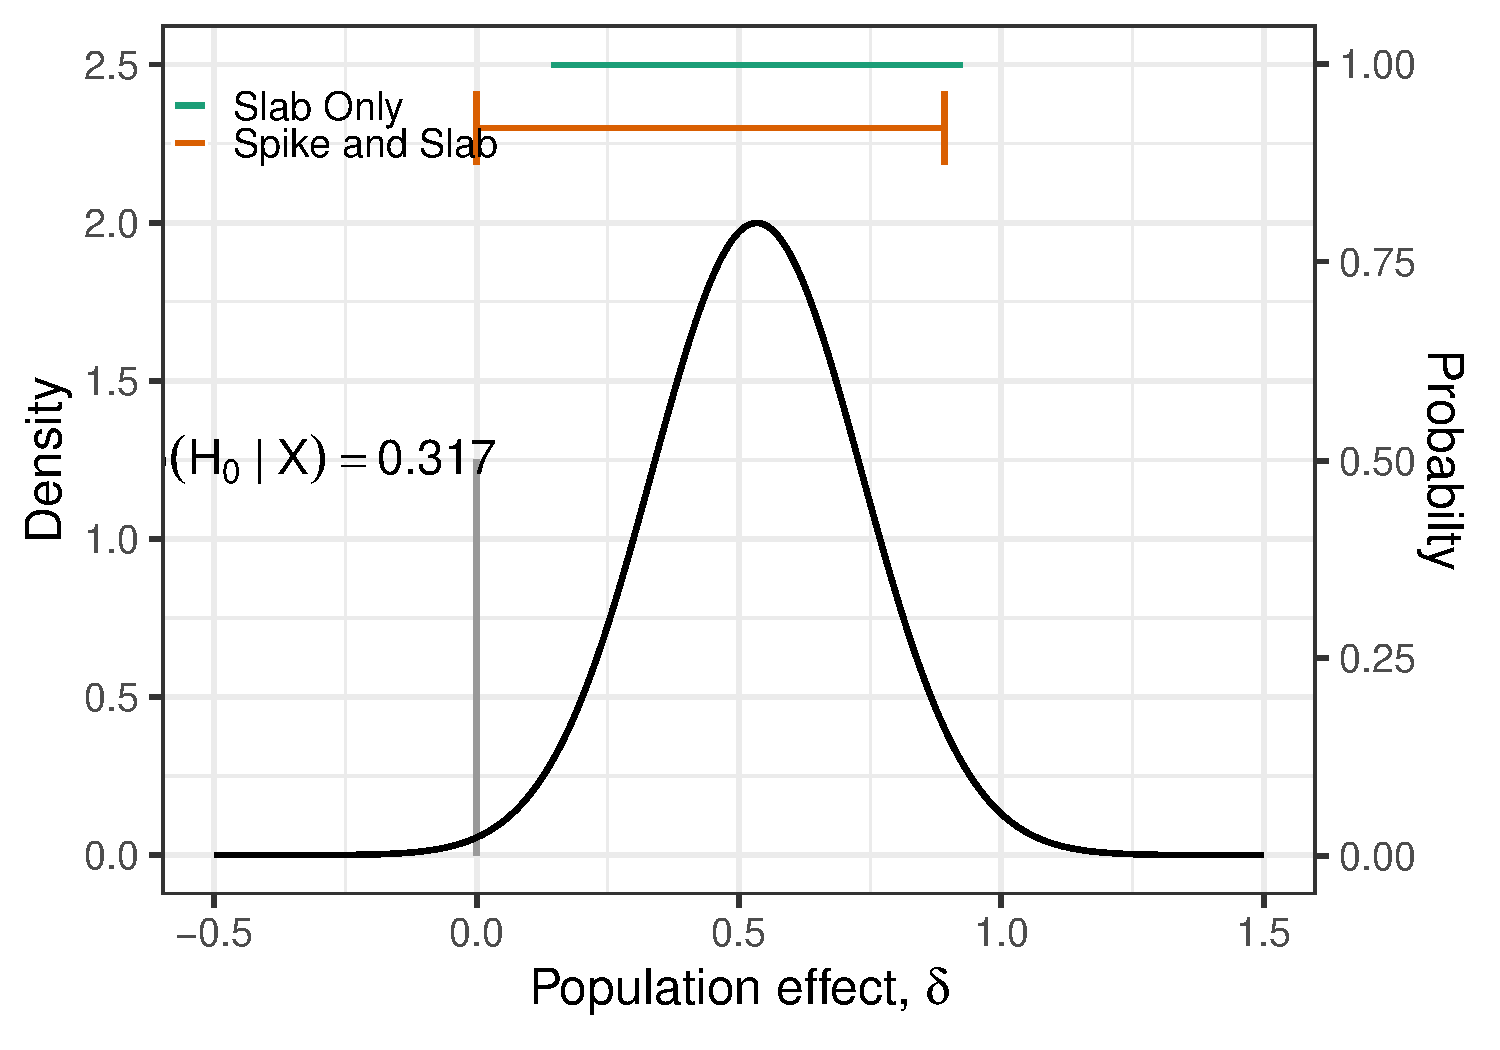
\includegraphics[width=\textwidth]{spikeAndSlabPosteriorRightAxis.pdf}
	\caption{A visualization of model averaging. The black line represents the posterior of the effect size given the alternative model (i.e., the slab). This posterior distribution integrates to the posterior probability of the model given uniform prior model probabilties. The grey line represent the posterior probability of the null model (i.e., the spike). The yellow error bar shows a 95\% central credible interval if inference is only based on the posterior under the slab. The purple error bar shows a 95\% central credible interval if inference is based on the model averaged posterior distribution. Although there is substantial uncertainty about the models ($p(\model_0\mid X) = p(\model_1\mid X) = 0.5$), an estimate based on only the posterior distribution of the alternative model may be overconfident and positively biased.}
	\label{fig:modelAveragedPosterior}
\end{figure}

\begin{figure}[!ht]
	\includegraphics[width=\textwidth]{posteriorMeanVsSampleDelta.pdf}
	\caption{Posterior mean for effect size (y-axis) as a function of the observed effect size (x-axis). The left panel shows inference conditional on the alternative model (i.e., the slab). The right panel shows the model averaged posterior mean, which shrinks towards 0 as the sample effect size approaches 0 and the null model becomes more plausible. The colors and line types represent different variances of the prior distribution.}
	\label{fig:posteriorMeanVsSampleDelta}
\end{figure}


Show prior-posterior plot from JASP:
With sparse data, the prior distribution on effect size will shrink the estimate towards 0. Happens with the default settings, but even more when the width is smaller.

Also, show spike at zero (maybe we need better JASP plot, will ask Don to create it):

The impact of H0 will shrink the estimate toward 0. This is most clear when H0 is a priori very likely (''plants do not grow faster when you pray for them'') or when the sample effect is very close to zero, so that it becomes clear that H0 might provide a more reasonable explanation.

Mention earlier literature:
Model averaging effect size:
\cite[pp. 640-641]{ZellnerVandaele1975}, as described in \cite[p. 600-601]{ZellnerSiow1980}; also \cite[p. 57]{Haldane1932}, \cite{IversonEtAl2010}

Early ideas that are conceptually similar can be found in \cite[p. 387]{WrinchJeffreys1921} (show BMA between $\mathcal{H}_1$ and $\mathcal{H}_0$ -- but for prediction, not estimating effect size!; see also \cite{Jevons18741913}).

See also \cite{RouderEtAl2018PBR}:

Key is Figure 5. The spike-and-slab model shows shrinkage towards zero for small observed effect sizes because the spike has increased influence.

``There are alternative interpretations that we find somewhat cumbersome. One is that the spike-and-slab can be viewed not as a model but as a model-averaging device. Here, the goal is not so much to define categories of effect and no-effect, but to average across both of them, and this averaging results in regularization. If one uses this interpretation, the prior odds settings are important as they influence the posterior weight given to each model component in the averaging. Another alternative interpretation comes from Kruschke and Liddell (Kruschke, 2011; Kruschke \& Liddell, 2017; this issue). Here, the spike and slab are seen as separate components in a hierarchical model. Accordingly, a focus on Bayes factors denotes a focus on the choice between components; a focus on posterior estimation entails parameter estimation after choosing the slab. We find this view difficult inasmuch as there is no a priori reason to choose the slab to focus on estimation. If one admits the possibility of the spike, then assuredly it should affect posterior estimation as well.''


\section*{Discussion}

Bayesian estimators more likely to underestimate the effect size, as prior mean is typically centered around the null which pulls the posterior mean towards 0.

\newpage
\clearpage
\bibliographystyle{apacite}
\bibliography{referenties}
%\clearpage

%\appendix
%\section{Bla}

\end{document}